%================================================
% CHAPTER 1: RELEASE 1 - SOFTWARE FOUNDATIONS AND ORCHESTRATION ENGINE
%================================================

\chapter{Release 1: Software Foundations and Orchestration Engine Deployment}
%================================================

\section{Introduction}
This chapter details the realisation of Release 1, which constitutes the fundamental foundation and engineering core of the ATB BI platform dedicated to customer risk management. The development of this version was divided into two sprints (Sprint 1 and Sprint 2) driven according to the Scrum methodology. The main objective of this first iteration is twofold: automate the creation of a secure environment (authentication, RBAC) and deploy the central orchestration engine (Apache Airflow), the true autonomous conductor of the system, capable of piloting the entire infrastructure without human intervention.

%================================================
\section{Sprint 1: Setting up the Environment, Security and Profiles}
%================================================

\subsection{Sprint 1 Presentation}
This first development increment establishes the security and environmental foundations of the banking platform. The major technical challenge lies in the total automation of the deployment (via Runbooks) and in the strict segregation of access between the different hierarchical levels of the bank (Central General Management, Risk Manager, Branch Manager).

The objective is to provide a robust installation script (\texttt{MASTER\_DEPLOYMENT\_RUNBOOK}) which configures the Python virtual environment, manages dependencies and initialises the security database. The front-end software interface is developed under the \textbf{Streamlit} framework, with asynchronous management of user sessions (\textit{st.session\_state}) to guarantee the security of future accesses.

%------------------------------------------------
\subsection{Sprint Backlog}

Table \ref{tab:sprint1_backlog} details the functional requirements selected for this first sprint, formalised as User Stories.

\begin{table}[H]
\centering
\caption{Sprint Backlog of Sprint 1}
\label{tab:sprint1_backlog}
\renewcommand{\arraystretch}{1.6}
\resizebox{\textwidth}{!}{
\begin{tabular}{|c|c|p{3cm}|p{6cm}|p{4.5cm}|}
\hline
\rowcolor{blue!15}
\textbf{ID} & \textbf{Priority} & \textbf{As a...} & \textbf{I want to...} & \textbf{So that...} \\
\hline
\textbf{US 1} & High & User (All Roles) & authenticate via a secure login interface & I can access my role-restricted analytical workspace safely. \\
\hline
\textbf{US 2} & High & Central General Management & create, modify, or deactivate user accounts in the console & I can control who has access to the platform (e.g. adding new Branch Managers). \\
\hline
\end{tabular}
}
\end{table}

%------------------------------------------------
\subsection{Global Modelling}

\subsubsection{Global Use Case Diagram of Sprint 1}

The use case diagram (Figure \ref{fig:uc_sprint1}) models the initial interactions of the actors with the system. The "Authenticate" use case is a mandatory passage point (\textit{include}) for any access to the application.

\begin{figure}[H]
\centering
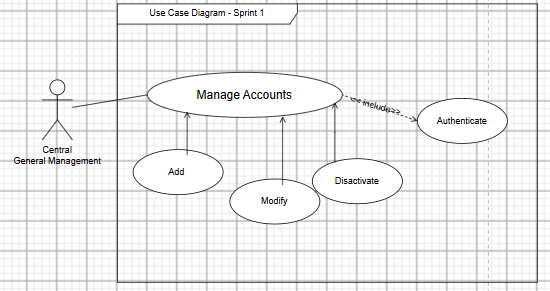
\includegraphics[width=0.9\textwidth]{figures/UseCaseDiagramSprint1.png}
\caption{Global use case diagram of Sprint 1}
\label{fig:uc_sprint1}
\end{figure}

\subsubsection{Class Diagram of Sprint 1}

The class diagram (Figure~\ref{fig:class_sprint1}) illustrates the role-based inheritance structure implemented in the security layer. The base \texttt{User} class defines common attributes such as \texttt{id}, \texttt{username}, \texttt{email}, \texttt{password\_hash}, \texttt{role}, and \texttt{status}. Three specialised subclasses inherit from it: \texttt{DGCentrale} (Central General Management) with administrative privileges, \texttt{RiskManager} for risk oversight, and \texttt{BranchManager} for agency-level access. The \texttt{AuthManager} class handles authentication logic and interacts with the \texttt{User} class to validate credentials and manage sessions.

\begin{figure}[H]
\centering
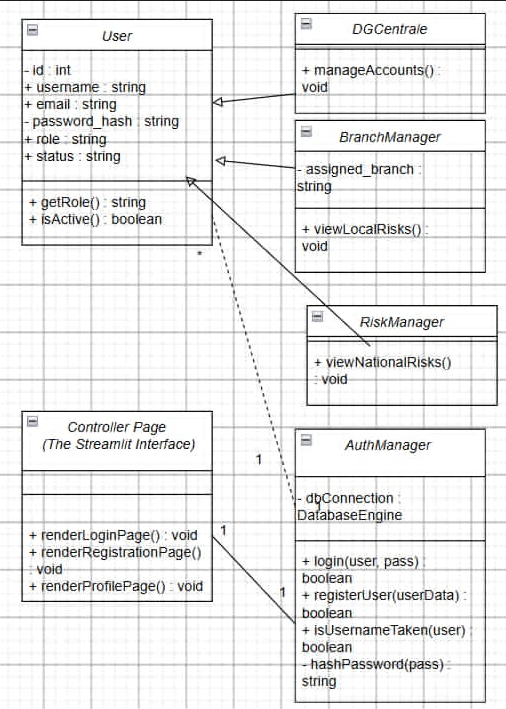
\includegraphics[width=0.82\textwidth]{figures/ClassDiagramSprint1.png}
\caption{Class diagram of Sprint 1 with Role Inheritance}
\label{fig:class_sprint1}
\end{figure}
The diagram makes explicit that authentication and session rights are centralised in
\texttt{AuthManager}, while business roles specialise a shared \texttt{User} base --- the
foundation of the RBAC model used throughout the dashboard.

%------------------------------------------------
\subsection{Use Case Refinement}

To validate compliance with the software architecture, the two main use cases of Sprint 1 are described in detail below.

\paragraph{Use Case Analysis: ``Authenticate''}

\begin{table}[H]
\centering
\caption{Textual description: Authenticate}
\label{tab:uc_auth}
\renewcommand{\arraystretch}{1.2}
\resizebox{\textwidth}{!}{
\begin{tabular}{|p{4cm}|p{11cm}|}
\hline
\rowcolor{blue!15}
\textbf{Use Case} & \textbf{Authenticate} \\
\hline
\textbf{Objective} & Secure dashboard access by verifying credentials against the relational database and establishing the session perimeter. \\
\hline
\textbf{Actor} & Central General Management, Branch Manager, Risk Manager \\
\hline
\textbf{Precondition} & The user possesses an active record in the database schema \texttt{PFE\_AUTH}. \\
\hline
\textbf{Postcondition} & The session variable \texttt{st.session\_state["auth\_user"]} is populated. \\
\hline
\textbf{Nominal Scenario} & 
1. The user connects to the Streamlit gateway page. \newline
2. The user enters their Username and Password. \newline
3. \texttt{AuthManager} hashes the password: $\text{SHA-256}(\text{"ATB\_BI\_2026:"} + \text{password})$. \newline
4. The system queries SQL Server table \texttt{PFE\_AUTH.dashboard\_users} using a parameterised statement. \newline
5. If the record matches, the user's display name, role key, and page rights are loaded. \newline
6. The user is redirected to their default home page dashboard. \\
\hline
\textbf{Alternative Scenario} & 
--- \textbf{Inactive User account} (\texttt{is\_active = 0}): Display *"Access denied. Account is inactive."* \newline
--- \textbf{Invalid Credentials}: Display *"Incorrect username or password."* \\
\hline
\end{tabular}
}
\end{table}

\begin{figure}[H]
\centering
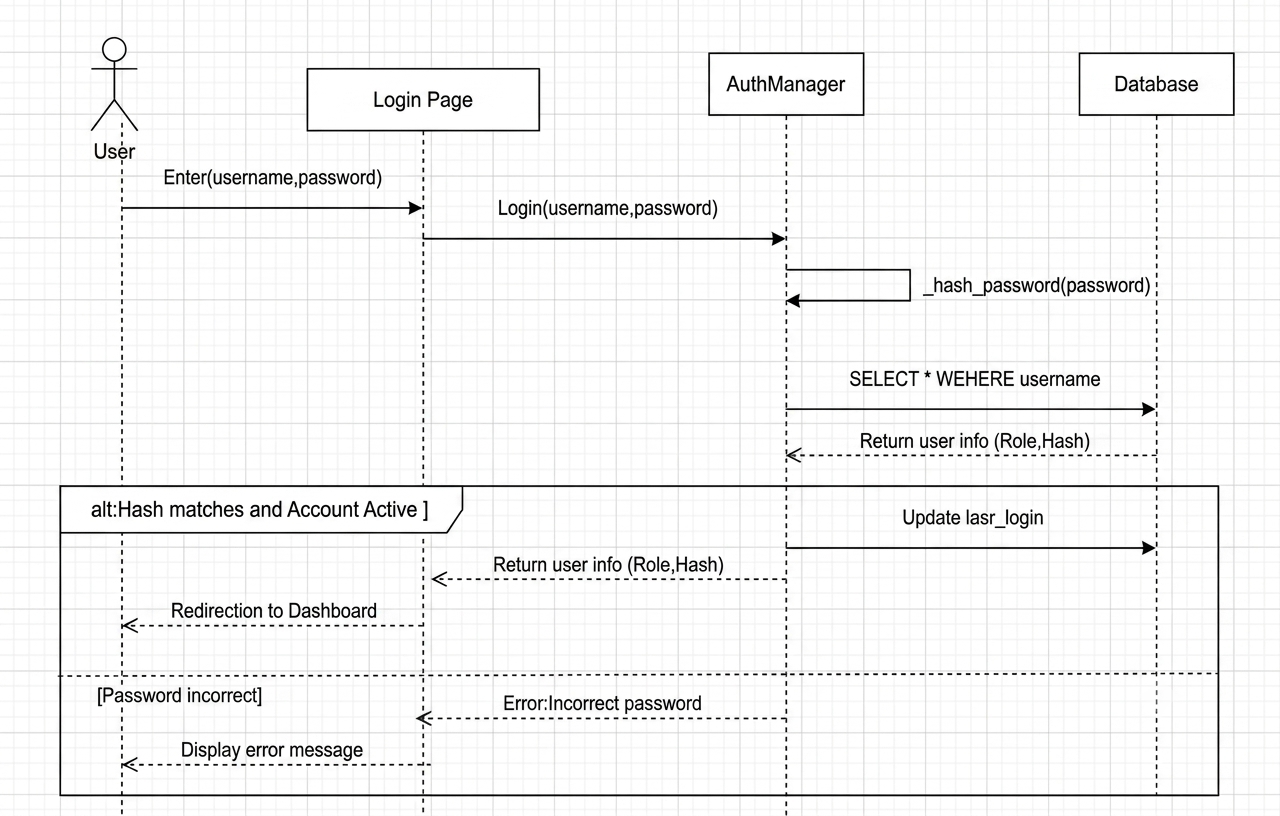
\includegraphics[width=0.85\textwidth,height=0.48\textheight,keepaspectratio]{figures/SequanceDiagramSprint1.png}
\caption{Sequence diagram: User Login}
\label{fig:seq_auth}
\end{figure}
The sequence shows credential capture on the login page, password hashing in
\texttt{AuthManager}, database lookup, and the success/failure alternatives that either
redirect to the dashboard or display an error.

\paragraph{Use Case Analysis: ``Manage Accounts''}

\begin{table}[H]
\centering
\caption{Textual description: Manage Accounts}
\label{tab:uc_manage_accounts}
\renewcommand{\arraystretch}{1.2}
\resizebox{\textwidth}{!}{
\begin{tabular}{|p{4cm}|p{11cm}|}
\hline
\rowcolor{blue!15}
\textbf{Use Case} & \textbf{Manage Accounts (Add/Modify/Deactivate)} \\
\hline
\textbf{Objective} & Allow the administrator (Central GM) to manage the cohort of platform users. \\
\hline
\textbf{Actor} & Central General Management \\
\hline
\textbf{Precondition} & The logged-in user possesses the role code \texttt{DG\_CENTRAL}. \\
\hline
\textbf{Postcondition} & The table \texttt{PFE\_AUTH.dashboard\_users} reflects the transaction. \\
\hline
\textbf{Nominal Scenario} & 
1. The administrator navigates to the "User Administration Console" page. \newline
2. They fill in the registration details (Username, Email, Display Name, Role, and optional Branch/DAO area). \newline
3. \texttt{AccountManager} checks for username uniqueness. \newline
4. \texttt{AccountManager} inserts the new record into the database. \newline
5. The administration table is dynamically refreshed. \\
\hline
\textbf{Alternative Scenario} & 
--- \textbf{Duplicate Detected}: Error message *"This username is already taken."* \\
\hline
\end{tabular}
}
\end{table}

\begin{figure}[H]
\centering
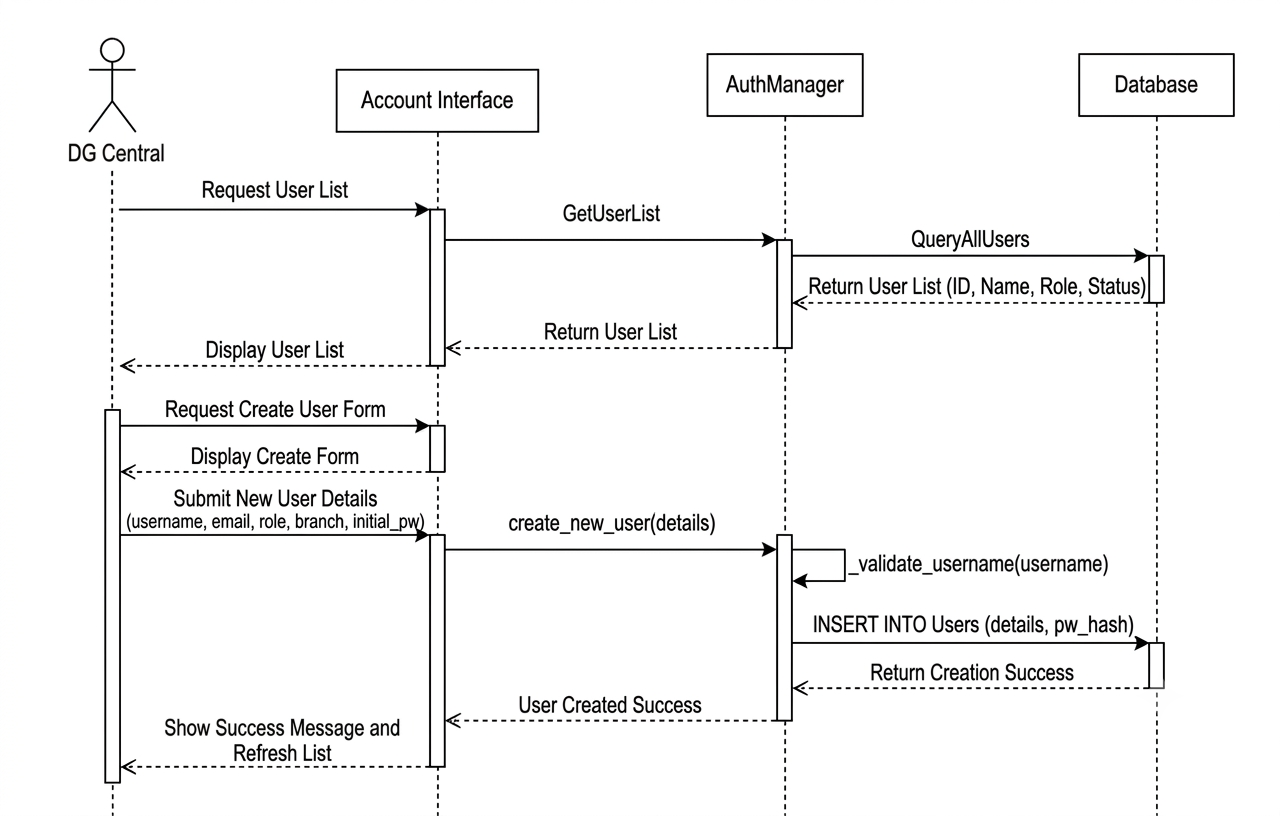
\includegraphics[width=0.85\textwidth,height=0.48\textheight,keepaspectratio]{figures/Sequance2DiagramSprint1.png}
\caption{Sequence diagram: Add New User via mangement}
\label{fig:seq_manage_accounts}
\end{figure}
This second sequence covers account creation and update by Central GM: uniqueness checks,
persistence in \texttt{PFE\_AUTH.dashboard\_users}, and refresh of the administration table.

%------------------------------------------------
\subsection{Sprint 1 Realisation}

The technical implementation of this sprint has been materialised through two distinct layers: database setup and application-level routing. The database schema PFE\_AUTH is configured in SQL Server using the setup\_auth.sql script. This script establishes the relational structures for system roles and the dashboard pages.

The application connects to SQL Server utilizing the SQLAlchemy engine configured with the pyodbc dialect using connection pooling parameters. Password verification is performed securely using Python's hashlib library by encoding the password payload combined with the custom cryptographic salt before running SHA-256. 

User session variables are managed securely via Streamlit's Session state. For Branch Managers, row-level data access is locked dynamically using the Branch filters helper, which appends geographic scopes directly to downstream analytical SQL queries, maintaining absolute security isolation.

\begin{figure}[H]
\centering
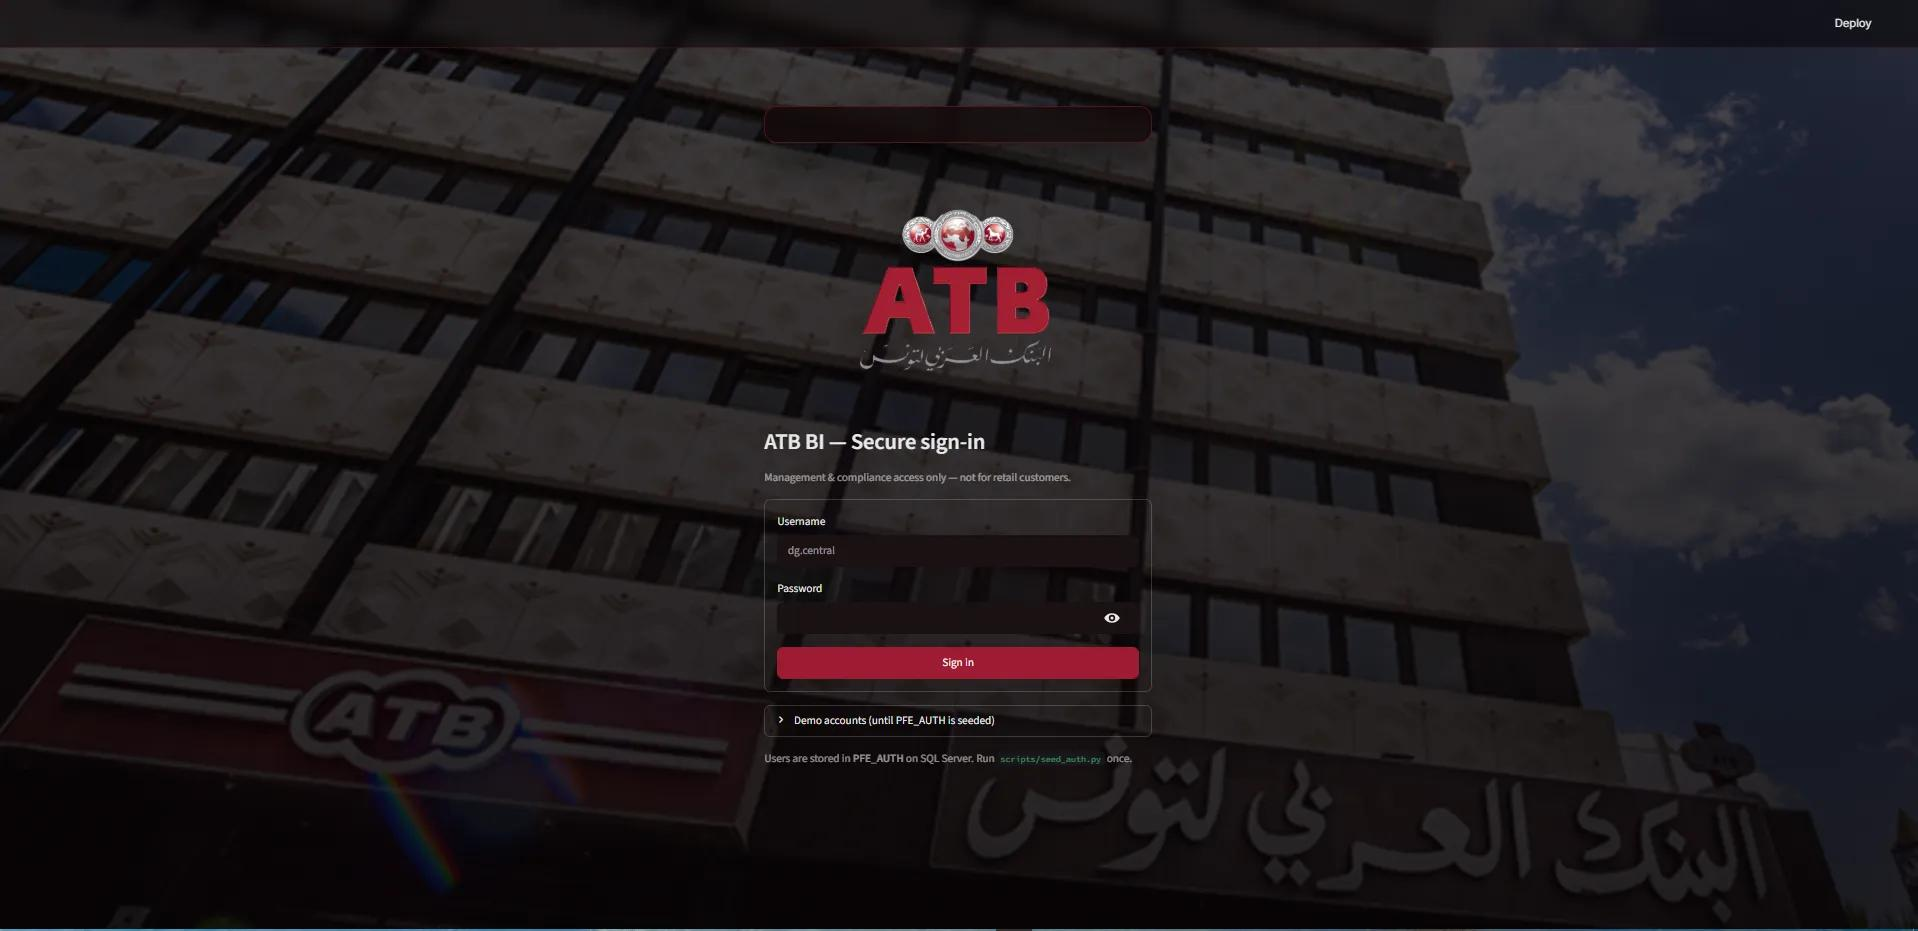
\includegraphics[width=0.85\textwidth]{figures/login_streamlit.png}
\caption{Interface: Secure authentication page (Streamlit)}
\label{fig:ui_login}
\end{figure}
The login gateway is the mandatory entry point for every role: credentials are verified
against \texttt{PFE\_AUTH} before any analytical page is exposed.

\begin{figure}[H]
\centering
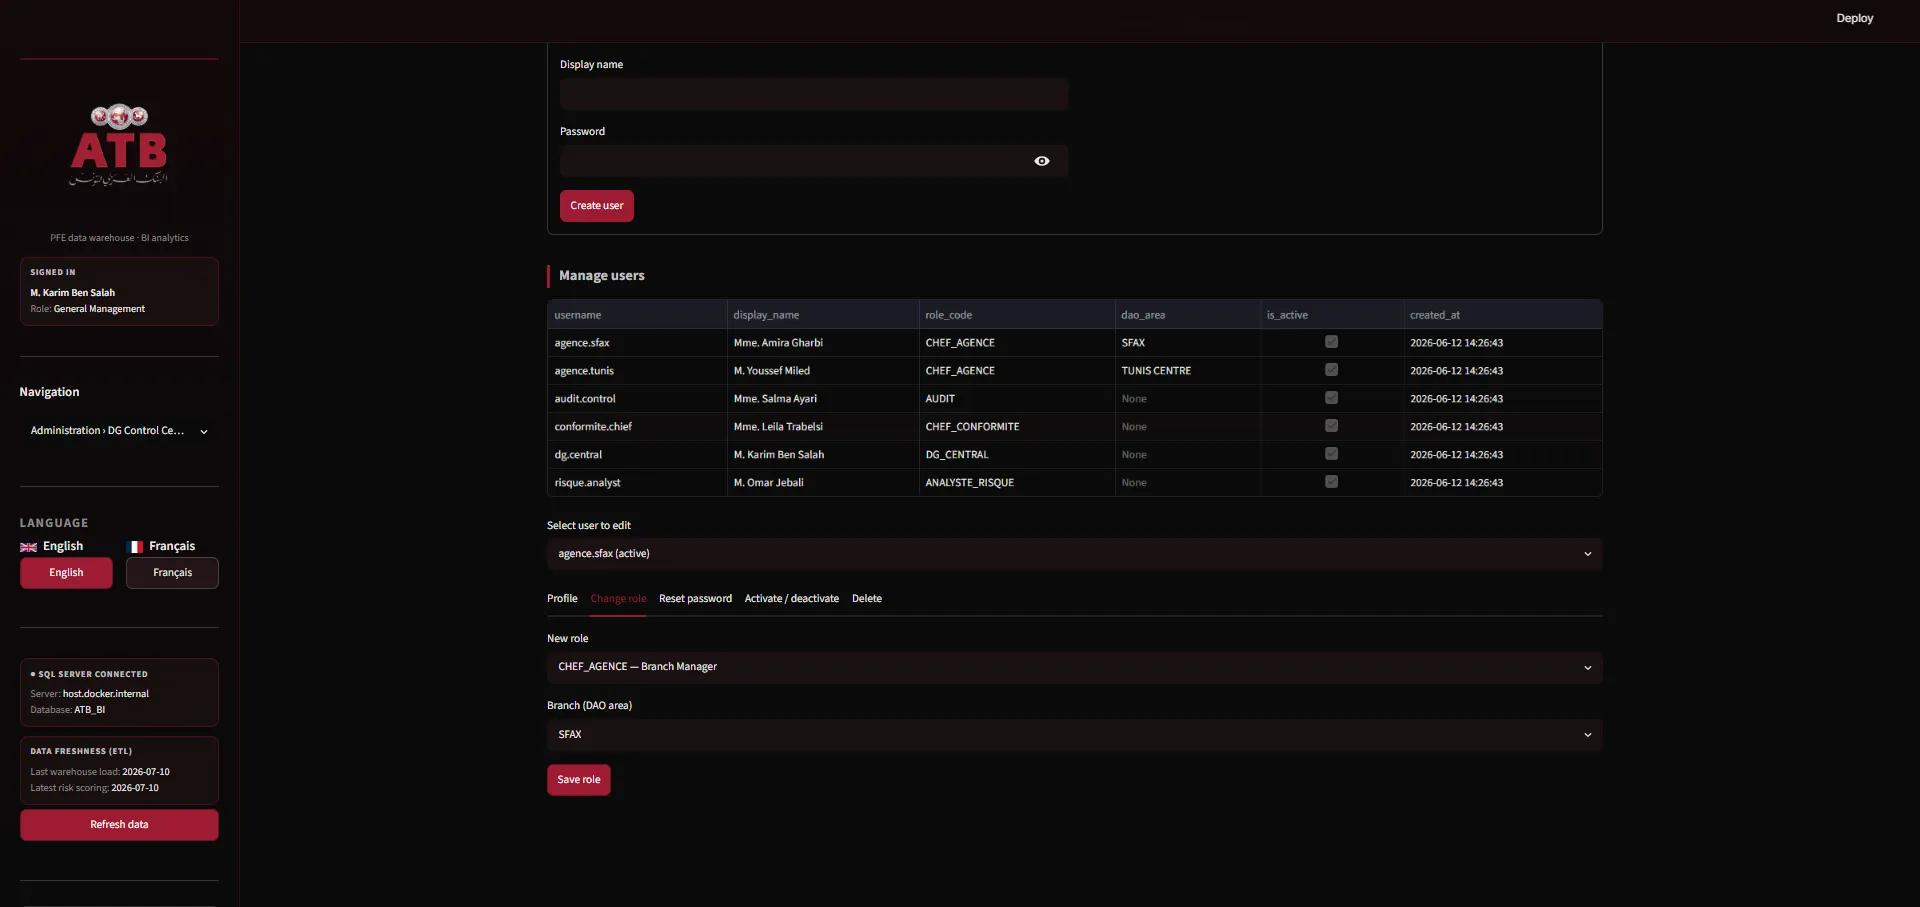
\includegraphics[width=0.85\textwidth]{figures/admin_panel.png}
\caption{Interface: Administration panel for Central GM}
\label{fig:ui_admin}
\end{figure}
Central General Management can create, update and deactivate dashboard users from this
console, enforcing US~02 without direct SQL access.

\begin{figure}[H]
\centering
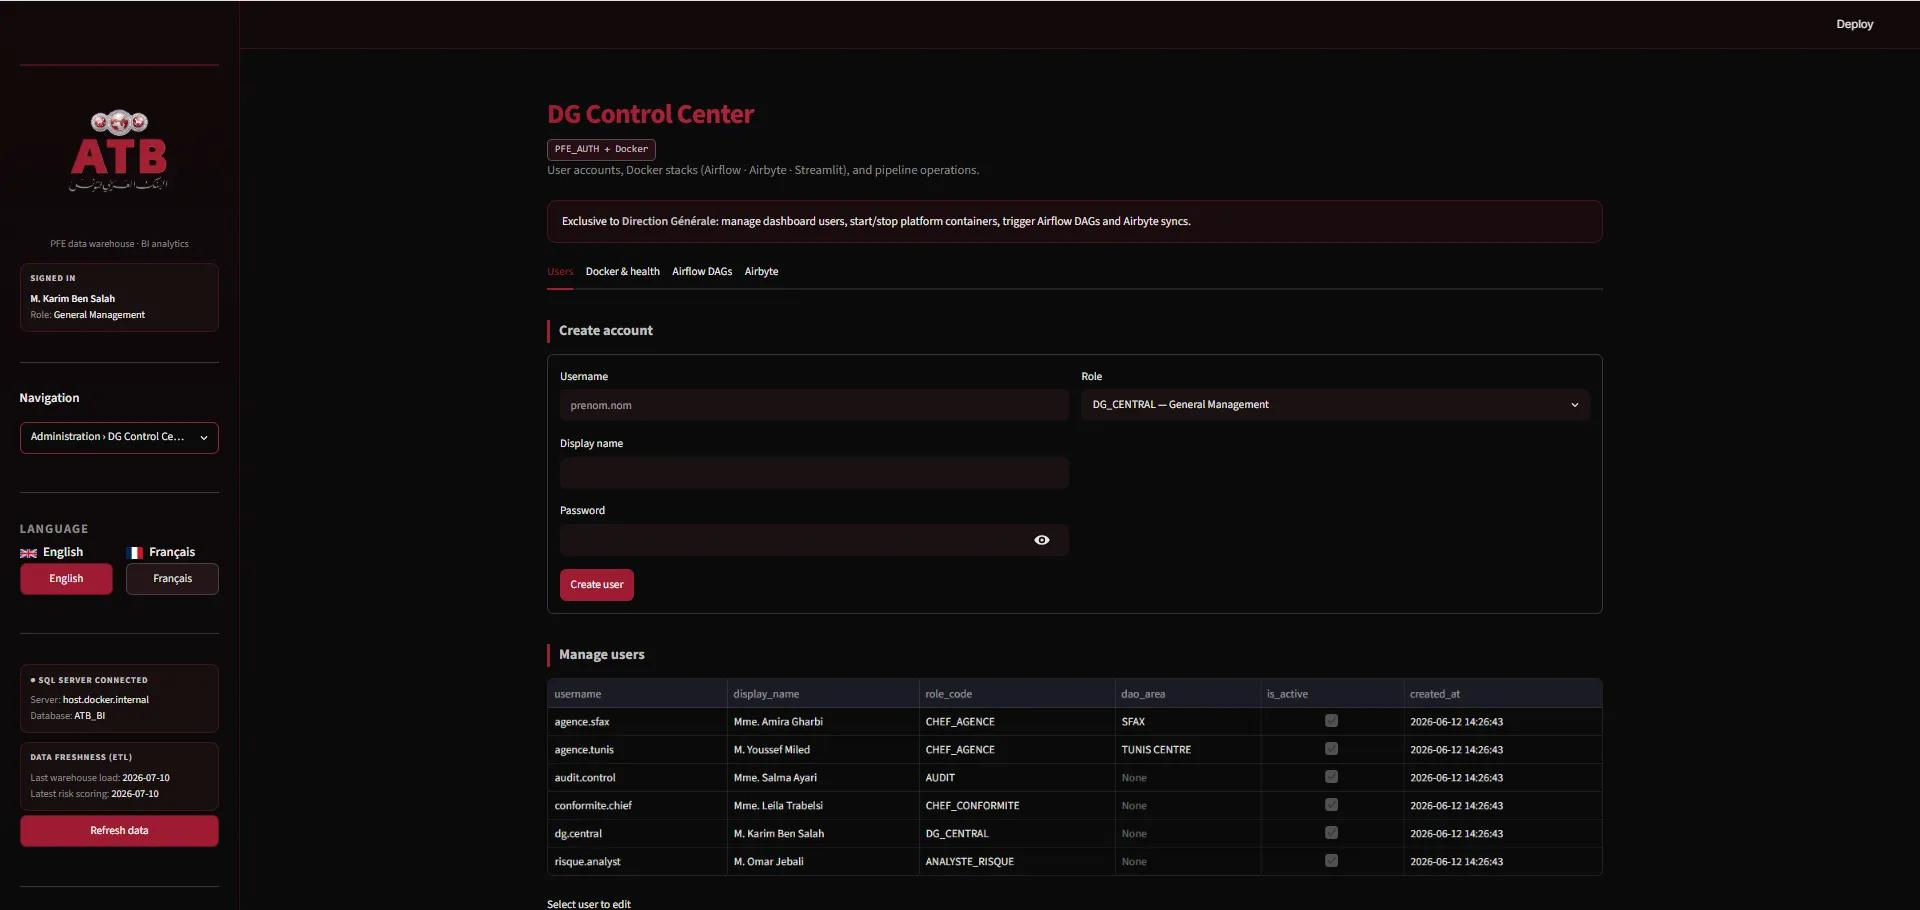
\includegraphics[width=0.85\textwidth]{figures/admin_panel2.png}
\caption{Interface: Detailed administration panel for Central GM}
\label{fig:ui_admin_detail}
\end{figure}
The detailed view lists active accounts with role and branch scope, confirming that
session rights and DAO filters remain consistent after each administration change.
%================================================
\section{Sprint 2: Deploying the Orchestration Engine}
%================================================

\subsection{Sprint 2 Overview}

With the software foundation secured and authenticated during Sprint 1, this second
sprint confronts the deeper challenge: making the platform \textit{think and act on
its own}. A data architecture is only as valuable as its ability to deliver fresh,
reliable information — consistently, automatically, and without depending on a human
to press a button each morning.

Without an orchestration layer, even the most sophisticated data pipeline is little
more than a collection of scripts that someone has to remember to run. In a banking
environment, where decisions are made daily on the basis of financial indicators, that
kind of fragility is simply unacceptable. Data must arrive on time, every time.

This sprint therefore focuses on deploying and configuring \textbf{Apache Airflow}, a
professional-grade workflow orchestration platform widely adopted across the data
engineering industry. Rather than running jobs manually or relying on fragile scheduled
scripts, Airflow allows the engineering team to define the entire data pipeline as a
structured programme — a \textbf{Directed Acyclic Graph (DAG)} — where each step knows
exactly what must happen before it, what it must produce, and what comes after it.

A critical architectural decision was made from the outset: the \textbf{entire
orchestration infrastructure is containerised using Docker}. Rather than installing
Airflow directly on a server — with all the configuration complexity, dependency
conflicts, and environment inconsistency that entails — every component runs inside
its own isolated Docker container, orchestrated together via Docker Compose. This
means the platform can be launched on any machine with a single command, the
environment is perfectly reproducible across development and production, and each
service is isolated from the others yet fully networked. Three dedicated containers
handle the workload: the \textbf{webserver} provides the browser-based monitoring
interface, the \textbf{scheduler} continuously watches the clock and triggers DAGs
at their configured times, and the \textbf{triggerer} manages long-running asynchronous
tasks. A fourth container runs a \textbf{PostgreSQL} database that stores Airflow's
own internal state — run history, task logs, variables, and connections — ensuring
that all operational data survives container restarts.

The pipeline runs automatically every night at 02:00 UTC, so that by the time
the first decision-maker opens the dashboard each morning, all data has already been
silently ingested, cleaned, transformed, validated, and loaded — with zero human
intervention required.

\begin{table}[H]
\centering
\renewcommand{\arraystretch}{1.4}
\caption{Key configuration parameters of the main orchestration pipeline}
\label{tab:dag_config}
\begin{tabular}{|p{4.5cm}|p{9cm}|}
\hline
\rowcolor{blue!15}
\textbf{Parameter} & \textbf{Value / Description} \\
\hline
Pipeline identifier & \texttt{atb\_bi\_warehouse\_etl} \\
\hline
Execution schedule & Every day at 02:00 UTC \\
\hline
Responsible team & Data Engineering \\
\hline
Automatic retries & 2 retries per task in case of failure \\
\hline
Retry delay & 5 minutes between each retry attempt \\
\hline
Failure notification & Automatic alert email sent to the engineering team \\
\hline
Concurrency control & Only one pipeline run active at a time \\
\hline
Historical backfill & Disabled — pipeline only processes current data \\
\hline
Classification tags & Production, ETL, Warehouse \\
\hline
\end{tabular}
\end{table}

%------------------------------------------------
\subsection{Sprint Backlog}

This sprint is built around a single, critical requirement but it is arguably the
most important one in the entire project. Everything built in Release 1 ultimately
serves this goal: a fully autonomous, self-managing data pipeline that guarantees
the daily freshness and integrity of banking data without any manual intervention.

\begin{table}[H]
\centering
\caption{Sprint Backlog of Sprint 2}
\label{tab:sprint2_backlog}
\renewcommand{\arraystretch}{1.6}
\resizebox{\textwidth}{!}{
\begin{tabular}{|c|c|p{3cm}|p{6cm}|p{4.5cm}|}
\hline
\rowcolor{blue!15}
\textbf{ID} & \textbf{Priority} & \textbf{As a\ldots} & \textbf{I want to\ldots} & \textbf{So that\ldots} \\
\hline
\textbf{US 3} & {\textbf{Very High}} &
Central General Management &
have the entire data pipeline orchestrated automatically, so that every stage —
ingestion, transformation, validation — runs without manual involvement &
the bank's data is always fresh, consistent, and trustworthy every single morning,
eliminating the risk of human error or forgotten executions. \\
\hline
\end{tabular}
}
\end{table}

%------------------------------------------------
\subsection{Global Modelling}

\subsubsection{(1) Use Case Diagram}

The use case diagram in Figure~\ref{fig:uc_sprint2} illustrates how the Central General
Management interacts with the orchestration system. The primary action — managing and
monitoring the automated pipeline — is accessible only after authentication, which
remains a mandatory precondition for accessing the Airflow control panel. This ensures
that even the operational monitoring interface is secured within the platform's access
control framework.

\begin{figure}[H]
\centering
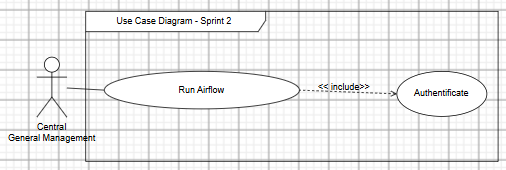
\includegraphics[width=0.9\textwidth]{figures/UseCaseDiagramSprint2.png}
\caption{Global use case diagram of Sprint 2}
\label{fig:uc_sprint2}
\end{figure}

\subsubsection{(2) Class Diagram: Airflow Pipeline Architecture}

Figure~\ref{fig:class_sprint2} represents the object-oriented structure underpinning
the pipeline. The design is organised into four main logical components, each with a
clearly defined responsibility: pipeline configuration and scheduling, task grouping
and dependency management, data quality verification, and runtime environment
configuration. This separation of concerns ensures that each part of the pipeline
can be maintained, tested, and modified independently.

\begin{figure}[H]
\centering
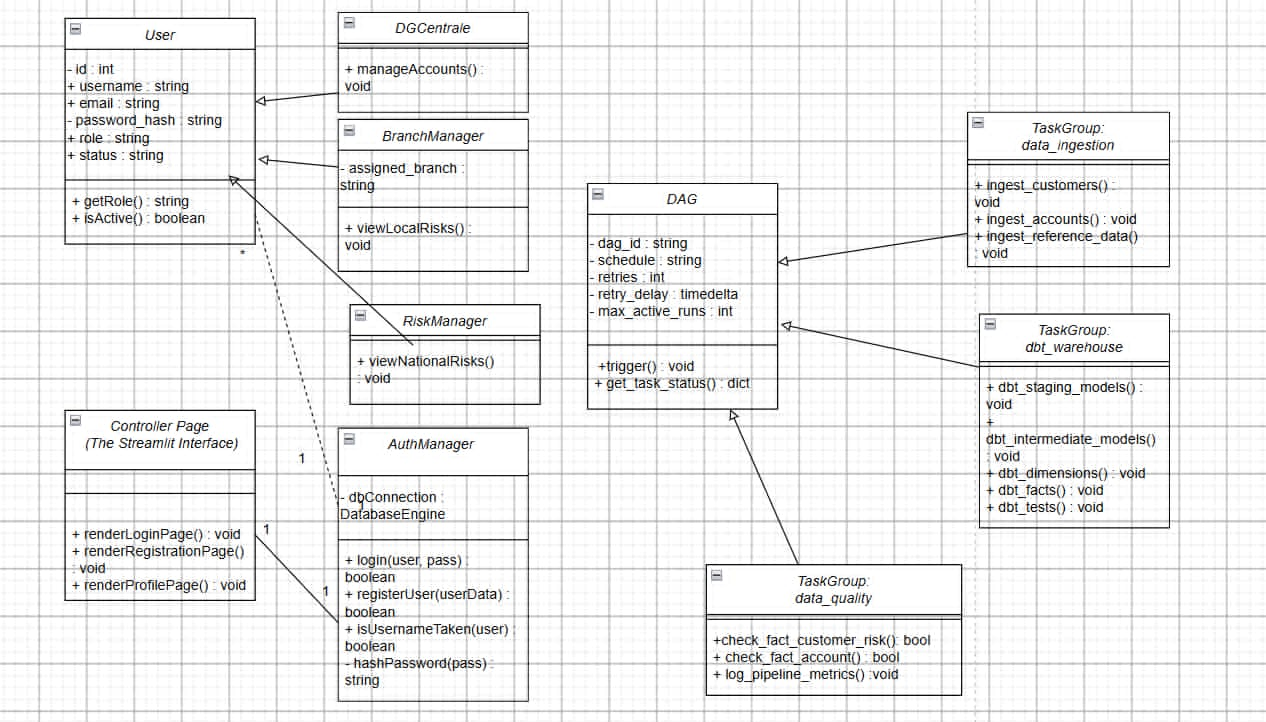
\includegraphics[width=0.9\textwidth]{figures/ClassDiagramSprint2.png}
\caption{Class diagram of Sprint 2 — Airflow DAG architecture}
\label{fig:class_sprint2}
\end{figure}

%------------------------------------------------
\subsection{Use Case Refinement}

\textbf{Use Case Analysis: ``Manage ETL (Airflow Orchestration)''}

\begin{table}[H]
\centering
\small
\caption{Textual description: Manage ETL (Airflow Orchestration)}
\label{tab:uc_airflow}
\renewcommand{\arraystretch}{1.2}
\resizebox{\textwidth}{!}{
\begin{tabular}{|p{3.5cm}|p{12.5cm}|}
\hline
\rowcolor{blue!15}
\textbf{Use Case} & \textbf{Manage ETL (Airflow Orchestration)} \\
\hline
\textbf{Objective} &
Supervise, monitor, and fully automate the banking data pipeline with
enterprise-grade reliability, ensuring consistent daily delivery of clean, validated
data with no manual intervention required. \\
\hline
\textbf{Actor} & Central General Management \\
\hline
\textbf{Precondition} &
The Airflow Docker stack is running and healthy. All required runtime
configuration variables such as the database connection details, the transformation
environment, and the notification endpoints  have been properly set up in Airflow's
configuration store. \\
\hline
\textbf{Postcondition} &
All pipeline tasks complete with a success status. Data quality checks confirm the
absence of any integrity violations across both fact tables. A full execution summary
is recorded and made available for review. \\
\hline
\textbf{Nominal Scenario} &
1. The nightly schedule fires automatically at 02:00 UTC. \newline
2. The pipeline initialises, logging the execution date and preparing the runtime context. \newline
3. \textbf{Data Ingestion:}Three parallel tasks simultaneously load data from
seven source files into the operational data store, maximising throughput. \newline
4. \textbf{Staging Transformation:} Raw ingested data is cleaned, standardised, and
cast into consistent formats, removing any noise introduced by the source systems. \newline
5. \textbf{Intermediate Transformation:}  Business logic is applied: risk pillars are
computed and relationships between entities are established. \newline
6. \textbf{Warehouse Loading:} Dimension tables are built first, followed by the two
central fact tables, respecting referential integrity at every step. \newline
7. \textbf{Schema Testing:}Automated tests verify that all constraints, data types,
and relationships are satisfied. \newline
8. \textbf{Data Quality Checks:}  Two independent verification tasks run in parallel,
probing both fact tables for NULL foreign keys and confirming that row counts meet
the expected minimum thresholds. \newline
9. \textbf{Metrics Logging:} Row counts and key indicators are aggregated into a
comprehensive execution summary, accessible to the engineering team. \newline
10. \textbf{Pipeline Completion:} The pipeline concludes successfully and optionally
triggers the downstream machine learning pipeline for further processing. \\
\hline
\textbf{Alternative Scenario} &
--- \textbf{Integrity violation detected}: If any NULL foreign key is found in a fact
table, the pipeline raises an error immediately, halting further execution and
triggering the automatic retry mechanism. \newline
--- \textbf{Insufficient data volume}: If a fact table contains fewer rows than the
defined minimum threshold, the pipeline treats this as a data anomaly, raises a
diagnostic error, and prevents downstream tasks from consuming potentially incomplete
data. \newline
--- \textbf{Transformation failure}: If a transformation step fails at any point, the
pipeline propagates the failure upward, blocks all dependent tasks, and dispatches an
automatic alert to the engineering team. \\
\hline
\end{tabular}
}
\end{table}

%------------------------------------------------
\subsection{Activity Diagram: Automated Pipeline Execution Flow}

The activity diagram in Figure~\ref{fig:activity_sprint2} models the control flow and
parallel execution branches of the \texttt{atb\_bi\_warehouse\_etl} pipeline. It details the
sequential stages --- from initial cron scheduling, parallel source ingestion into
\texttt{PFE\_ODS}, three-tier dbt transformations, parallel fact quality checks, to the conditional
downstream machine learning trigger.

\begin{figure}[H]
\centering
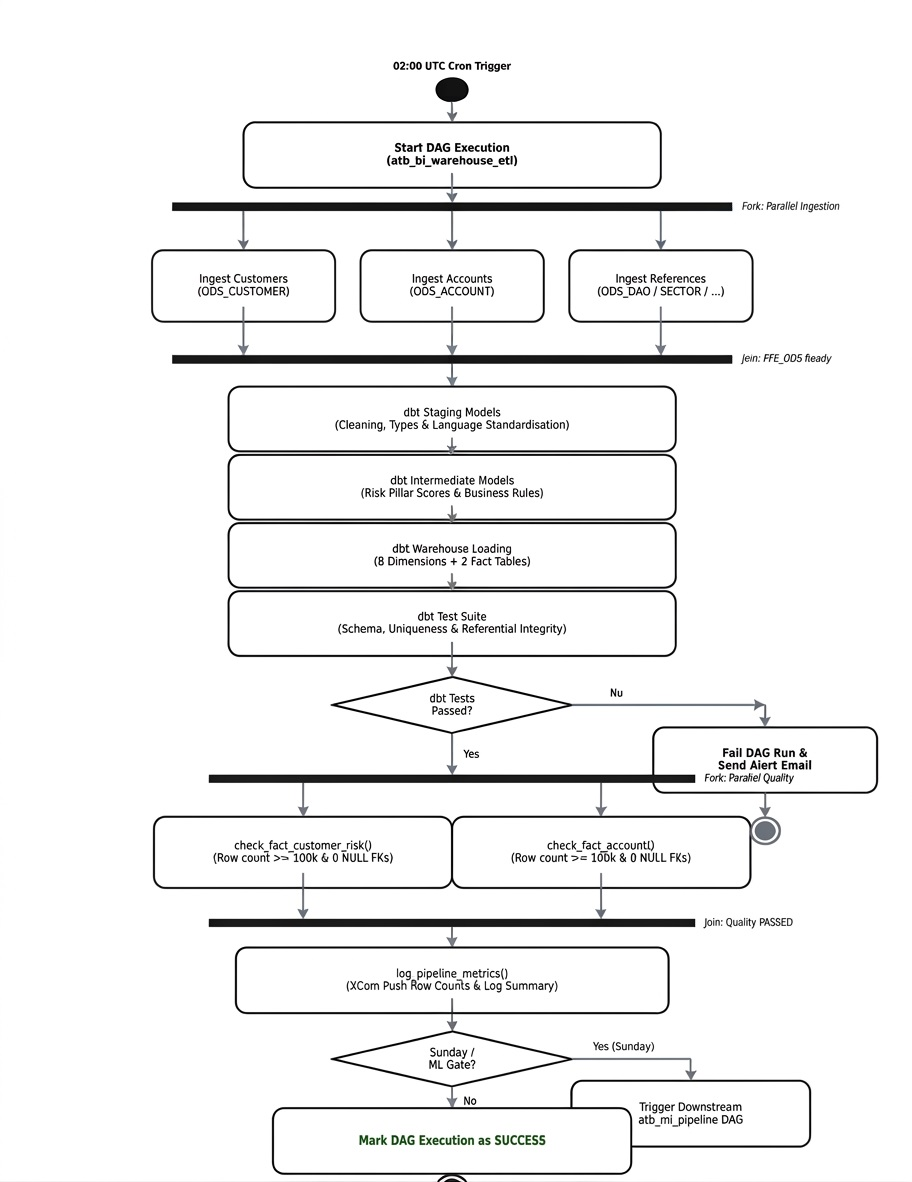
\includegraphics[width=0.7\textwidth]{figures/ActivityDiagramAIRFLOW1.png}
\caption{Activity diagram: end-to-end automated pipeline execution flow}
\label{fig:activity_sprint2}
\end{figure}

%------------------------------------------------
\subsection{Sprint 2 Realisation}

\subsubsection{Infrastructure: A Fully Containerised Platform and DevOps Work}

Before discussing what the pipeline does, it is important to understand \textit{how} it runs. A key engineering effort of this project was designing a custom containerised platform rather than relying on generic setups. 

The entire Airflow orchestration infrastructure is packaged as a \textbf{custom Docker image} (\texttt{atb-airflow:2.9.1}), defined in a dedicated \texttt{Dockerfile}. This custom image extends the official base distribution with:
\begin{itemize}
    \item Native Microsoft SQL Server ODBC Driver 17 for direct relational connectivity.
    \item \texttt{dbt-sqlserver} and transformation dependencies allowing Airflow tasks to run dbt models directly inside the container.
    \item Embedded Machine Learning execution packages (\texttt{xgboost}, \texttt{scikit-learn}, \texttt{mlflow}) to support automated retraining DAGs.
\end{itemize}

% --- SCREENSHOT: Add screenshot of 2_orchestration/Dockerfile here
\begin{figure}[H]
\centering
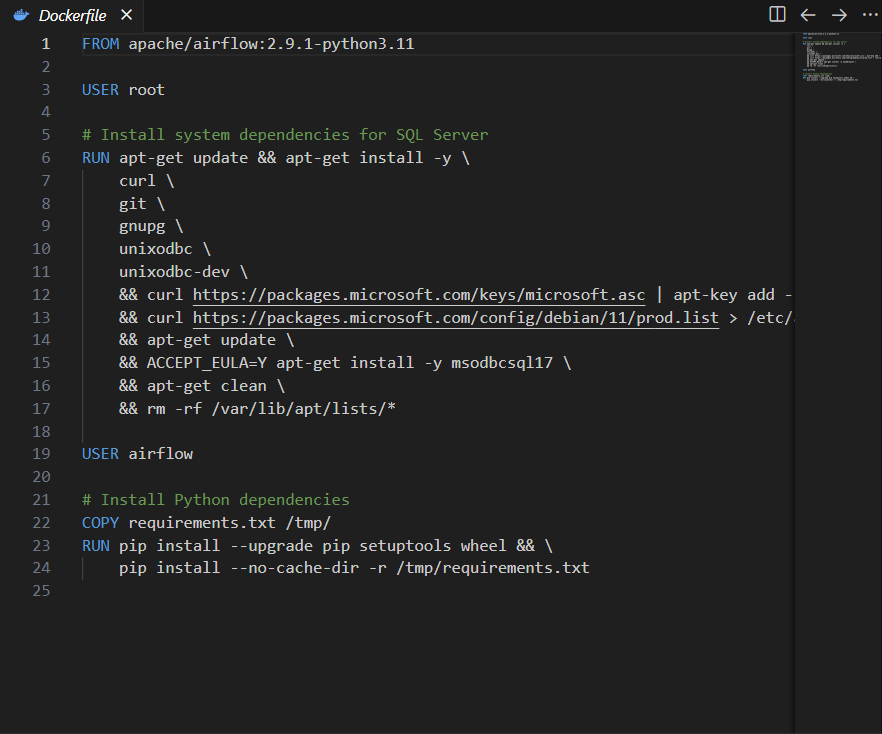
\includegraphics[width=0.88\textwidth]{figures/airflow_dockerfile_yaml.png}
\caption{Custom Dockerfile configuration for the ATB Airflow orchestration container}
\label{fig:airflow-dockerfile-code}
\end{figure}
\noindent Custom Dockerfile specification for the Airflow engine container.

The service architecture is defined in a custom \textbf{\texttt{docker-compose.yml}} specification that orchestrates four coordinated containers:

\begin{table}[H]
\centering
\small
\renewcommand{\arraystretch}{1.4}
\caption{Docker containers composing the Airflow orchestration stack}
\label{tab:docker_containers}
\begin{tabular}{|p{3.5cm}|p{10cm}|}
\hline
\rowcolor{blue!15}
\textbf{Container} & \textbf{Role} \\
\hline
\textbf{Airflow Webserver} &
Serves the browser-based monitoring interface on port 8080. This is where the
engineering team views DAG run histories, task logs, and pipeline status. \\
\hline
\textbf{Airflow Scheduler} &
The engine that watches the clock, evaluates which DAGs are due to run, and
dispatches tasks to available workers. It runs continuously in the background. \\
\hline
\textbf{Airflow Triggerer} &
Handles deferred tasks those that wait for an external event (such as a downstream
DAG completing) without occupying a worker slot. \\
\hline
\textbf{PostgreSQL Database} &
Stores all of Airflow's internal state: run history, task instance logs, variable
values, connection credentials, and user accounts. \\
\hline
\end{tabular}
\end{table}

% --- SCREENSHOT: Add screenshot of 2_orchestration/docker-compose.yml here
\begin{figure}[H]
\centering
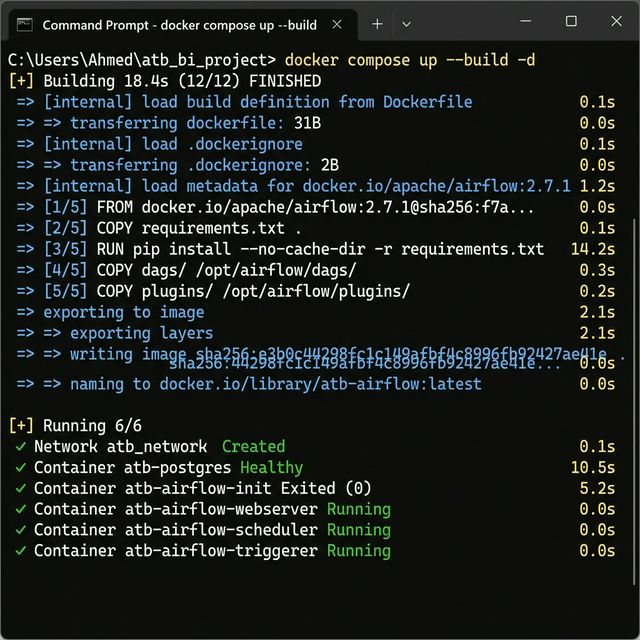
\includegraphics[width=0.88\textwidth]{figures/airflow_docker_compose_yaml.png}
\caption{Custom docker-compose.yml orchestration file for the Airflow stack}
\label{fig:airflow-docker-compose-yaml}
\end{figure}
\noindent % [USER INSTRUCTION]: Place your screenshot of 2_orchestration/docker-compose.yml above (uncomment \includegraphics).

All containers share a dedicated bridge network (\texttt{atb-network}) and connect to host-bound services via \texttt{host.docker.internal:host-gateway}. The transformation models, raw datasets, and ML sources are mounted as volumes into the containers, ensuring instant code updates without container rebuilds.
raw data files are mounted directly into the containers as volumes, so that updates to
the pipeline code take effect without needing to rebuild the image. The platform can
be brought up or torn down entirely in seconds.

\subsubsection{The DAG Ecosystem: Four Pipelines, One Platform}

One of the strengths of the Airflow implementation is that it does not rely on a single
monolithic pipeline. Instead, the engineering team designed a \textbf{family of four
complementary DAGs}, each with a distinct responsibility. Together they form a
layered orchestration ecosystem, where each DAG can operate independently or be
triggered as part of a larger chain.

\paragraph{DAG 1: The Master Pipeline}

This is the backbone of the entire platform and the DAG that runs every single night.
Designed as the comprehensive end-to-end orchestrator, it takes full ownership of the
data lifecycle from ingestion through transformation to machine learning, combining the
responsibilities of warehouse loading and production orchestration into a single,
authoritative pipeline.

The pipeline is built as a sequence of nine tasks organised into three task groups.
It begins by attempting to synchronise data via Airbyte the dedicated ingestion
platform and falls back gracefully if Airbyte is not configured, validating instead
that the operational data store already contains fresh data. A \textbf{parallel
ingestion phase} then loads customer data, account data, and all reference tables
(currencies, sectors, industries, organisational units, and risk targets) simultaneously.
Once ingestion is confirmed, a \textbf{three-layer transformation phase} takes over:
the staging layer cleans and standardises the raw data, the intermediate layer applies
business logic and computes risk indicators, and the warehouse layer first populates
eight dimension tables before building the two central fact tables on top of them.
A structural testing phase runs automatically to verify all constraints and data types,
followed by a \textbf{parallel data quality phase} that probes both fact tables for
NULL foreign keys and confirms row counts above the expected minimum threshold.
A full execution summary is then logged. Uniquely, the pipeline also includes a
\textbf{weekly machine learning gate}: every Sunday, after the warehouse is confirmed
clean, it automatically triggers the XGBoost risk model retraining ensuring the
ML model is refreshed with the most recent banking data every week without any manual
scheduling.

\paragraph{DAG 2: The Standalone Ingestion Pipeline}

This DAG handles data ingestion in isolation. It connects to Airbyte, triggers
synchronisation jobs for each of the seven data sources, waits for them to complete,
and then validates that the resulting data in the operational data store meets minimum
volume expectations. It is designed to be run manually when a fresh data load is
needed outside the normal nightly schedule, or to be called as a component by the
master pipeline when fine-grained control over the ingestion phase is required.

\paragraph{DAG 3: The Standalone Transformation Pipeline}

This DAG covers only the dbt transformation layer. It runs the full sequence of
transformation steps from a connection health check and dependency installation,
through all three model layers (staging, intermediate, warehouse) to a final round
of structural tests and automatic documentation generation. Its purpose is to allow
the engineering team to re-run transformations independently, for example after
correcting a model or deploying new business logic, without needing to re-trigger
the ingestion phase.

\paragraph{DAG 4: The Machine Learning Pipeline}

The final DAG in the ecosystem is dedicated entirely to the machine learning lifecycle.
It can be triggered manually or automatically from the master pipeline on a weekly
basis. It runs the XGBoost customer risk model training script, waits for it to
complete, verifies that the trained model artefact was produced correctly, and then
executes a separate script that writes the model's predictions back into the data
warehouse making them available for display in the Streamlit dashboard. The entire
ML refresh cycle, from training to warehouse update, is therefore fully automated
and requires no human involvement.

\begin{table}[H]
\centering
\small
\renewcommand{\arraystretch}{1.5}
\caption{Summary of DAGs deployed in the Airflow ecosystem}
\label{tab:dag_summary}
\begin{tabular}{|p{4.2cm}|p{2.5cm}|p{7.3cm}|}
\hline
\rowcolor{blue!15}
\textbf{DAG} & \textbf{Schedule} & \textbf{Purpose} \\
\hline
DAG~1 --- Master Pipeline & Daily 02:00 UTC & End-to-end pipeline: Airbyte sync → ingest → transform → test → validate → log → weekly ML trigger \\
\hline
DAG~2 --- Standalone Ingestion & On demand & Airbyte data synchronisation + ODS validation only \\
\hline
DAG~3 --- Standalone Transformation & On demand & Full dbt run across all three model layers + documentation generation \\
\hline
DAG~4 --- Machine Learning Pipeline & Weekly (Sunday) or on demand & XGBoost model retraining + prediction writing to data warehouse \\
\hline
\end{tabular}
\end{table}

\subsubsection{The Main Pipeline in Detail: Nine Steps, One Unbroken Chain}

The nightly warehouse ETL pipeline the DAG that runs automatically every day is
structured into \textbf{nine sequential phases}, logically grouped into three task
groups. This design balances parallelism, where independent tasks can run simultaneously
to save time, with strict ordering, ensuring that no downstream step ever begins before
its upstream dependencies have fully succeeded.

\begin{table}[H]
\centering
\small
\renewcommand{\arraystretch}{1.5}
\caption{Execution phases of the automated data pipeline}
\label{tab:dag_phases}
\begin{tabular}{|c|p{3.5cm}|p{4cm}|p{5cm}|}
\hline
\rowcolor{blue!15}
\textbf{Phase} & \textbf{Task / Group} & \textbf{Mechanism} & \textbf{Output} \\
\hline
1 & Pipeline Start & Shell command & Execution context initialised and logged \\
\hline
2 & \textbf{Data Ingestion} (parallel) & 3 simultaneous tasks & 7 source files loaded into the operational data store \\
\hline
3 & Staging Transformation & Shell command & Raw data cleaned and standardised \\
\hline
4 & Intermediate Transformation & Shell command & Business logic applied; risk pillars computed \\
\hline
5 & \textbf{Warehouse Loading} (sequential) & 2 ordered tasks & 8 dimension tables + 2 fact tables built.\\
\hline
6 & Schema \& Integrity Testing & Shell command & All structural and relational tests pass \\
\hline
7 & \textbf{Data Quality Checks} (parallel) & 2 simultaneous tasks & Zero NULL foreign keys confirmed on both fact tables \\
\hline
8 & Metrics Logging & Python function & Full execution summary produced \\
\hline
9 & Pipeline Completion & Shell command & Success confirmed; ML pipeline optionally triggered \\
\hline
\end{tabular}
\end{table}

The entire dependency structure of the pipeline is expressed in a single, readable
declaration that reflects the architecture at a glance:

\begin{center}
\small
\textit{Start $\rightarrow$ Data Ingestion $\rightarrow$ Staging $\rightarrow$ Intermediate $\rightarrow$ Warehouse $\rightarrow$ Testing $\rightarrow$ Quality Checks $\rightarrow$ Metrics $\rightarrow$ Success}
\end{center}

\subsubsection{Data Quality Framework: Trusting the Numbers}

One of the most critical aspects of a banking data platform is the ability to trust
the numbers it produces. A dashboard showing inaccurate figures is worse than no
dashboard at all  it leads to confident, well-presented errors. To prevent this,
the pipeline embeds a dedicated data quality verification layer that runs automatically
after every transformation cycle.

This layer performs a series of targeted checks against both fact tables, probing for
the specific categories of integrity failure most likely to arise from data ingestion
or transformation issues:

\begin{table}[H]
\centering
\small
\renewcommand{\arraystretch}{1.4}
\caption{Data quality checks embedded in the pipeline}
\label{tab:dq_checks}
\begin{tabular}{|p{4.5cm}|p{4cm}|p{5.2cm}|}
\hline
\rowcolor{blue!15}
\textbf{Check} & \textbf{Scope} & \textbf{Failure Condition} \\
\hline
Customer reference integrity & Both fact tables & Any unresolved customer link raises an error \\
\hline
Organisational unit integrity & Both fact tables & Any unresolved organisational reference raises an error \\
\hline
Currency reference integrity & Account fact table & Any unresolved currency reference raises an error \\
\hline
Industry classification integrity & Customer risk fact table & Any unresolved industry reference raises an error \\
\hline
Risk target reference integrity & Customer risk fact table & Any unresolved risk target reference raises an error \\
\hline
Minimum data volume & Both fact tables & Fewer than 100,000 rows triggers a data anomaly alert \\
\hline
\end{tabular}
\end{table}

When a check passes, it records its result so that the final reporting task can
aggregate all metrics into a single execution summary giving the engineering team
full visibility into every pipeline run, including exactly how many records were
processed across each table.

\subsubsection{Resilience by Design: Configuration and Fault Tolerance}

A production data platform must be both secure and resilient. On the security side,
no sensitive information such as database credentials, server addresses, or
notification endpoints is written directly into the pipeline code. Instead, all
configuration is stored separately in Airflow's secure variable store and injected
at runtime, so that the same pipeline code can run safely across different environments
without modification.

\begin{table}[H]
\centering
\small
\renewcommand{\arraystretch}{1.3}
\caption{Runtime configuration variables injected securely at pipeline execution}
\label{tab:airflow_vars}
\begin{tabular}{|p{4.5cm}|p{9cm}|}
\hline
\rowcolor{blue!15}
\textbf{Configuration Variable} & \textbf{Purpose} \\
\hline
Transformation project path & Tells the pipeline where to find the transformation models \\
\hline
Transformation profile & Identifies which transformation configuration set to use \\
\hline
Execution environment & Specifies whether the pipeline is running in production or development \\
\hline
Database server & Hostname of the target SQL Server instance \\
\hline
Target database & The name of the analytical data warehouse database \\
\hline
Notification endpoint & Webhook URL for real-time failure notifications \\
\hline
\end{tabular}
\end{table}

On the resilience side, every task in the pipeline is configured with a fault-tolerance
policy: if a task fails due to a transient issue a momentary network interruption,
a database timeout, or a brief resource constraint  Airflow will automatically retry
it up to two times, waiting five minutes between each attempt. This window is large
enough for most transient issues to self-resolve, and small enough that the pipeline
still completes well before the business day begins. If all retries are exhausted and
the task remains failed, an automatic alert is dispatched to the engineering team,
ensuring that no failure goes unnoticed.

\subsubsection{Bringing It All Together: The Integrated Monitoring Panel}

One of the most practically powerful features delivered in this sprint is the
\textbf{integration of Airflow monitoring directly into the Streamlit platform}. Rather
than requiring the engineering team or management to open a separate browser tab,
log into Airflow independently, and interpret its technical interface, the Streamlit
dashboard includes a dedicated \textbf{Operations Console} accessible exclusively
to users with the highest administrative privileges.

This console is designed to answer one simple question: \textit{is everything working?}

\begin{figure}[H]
\centering
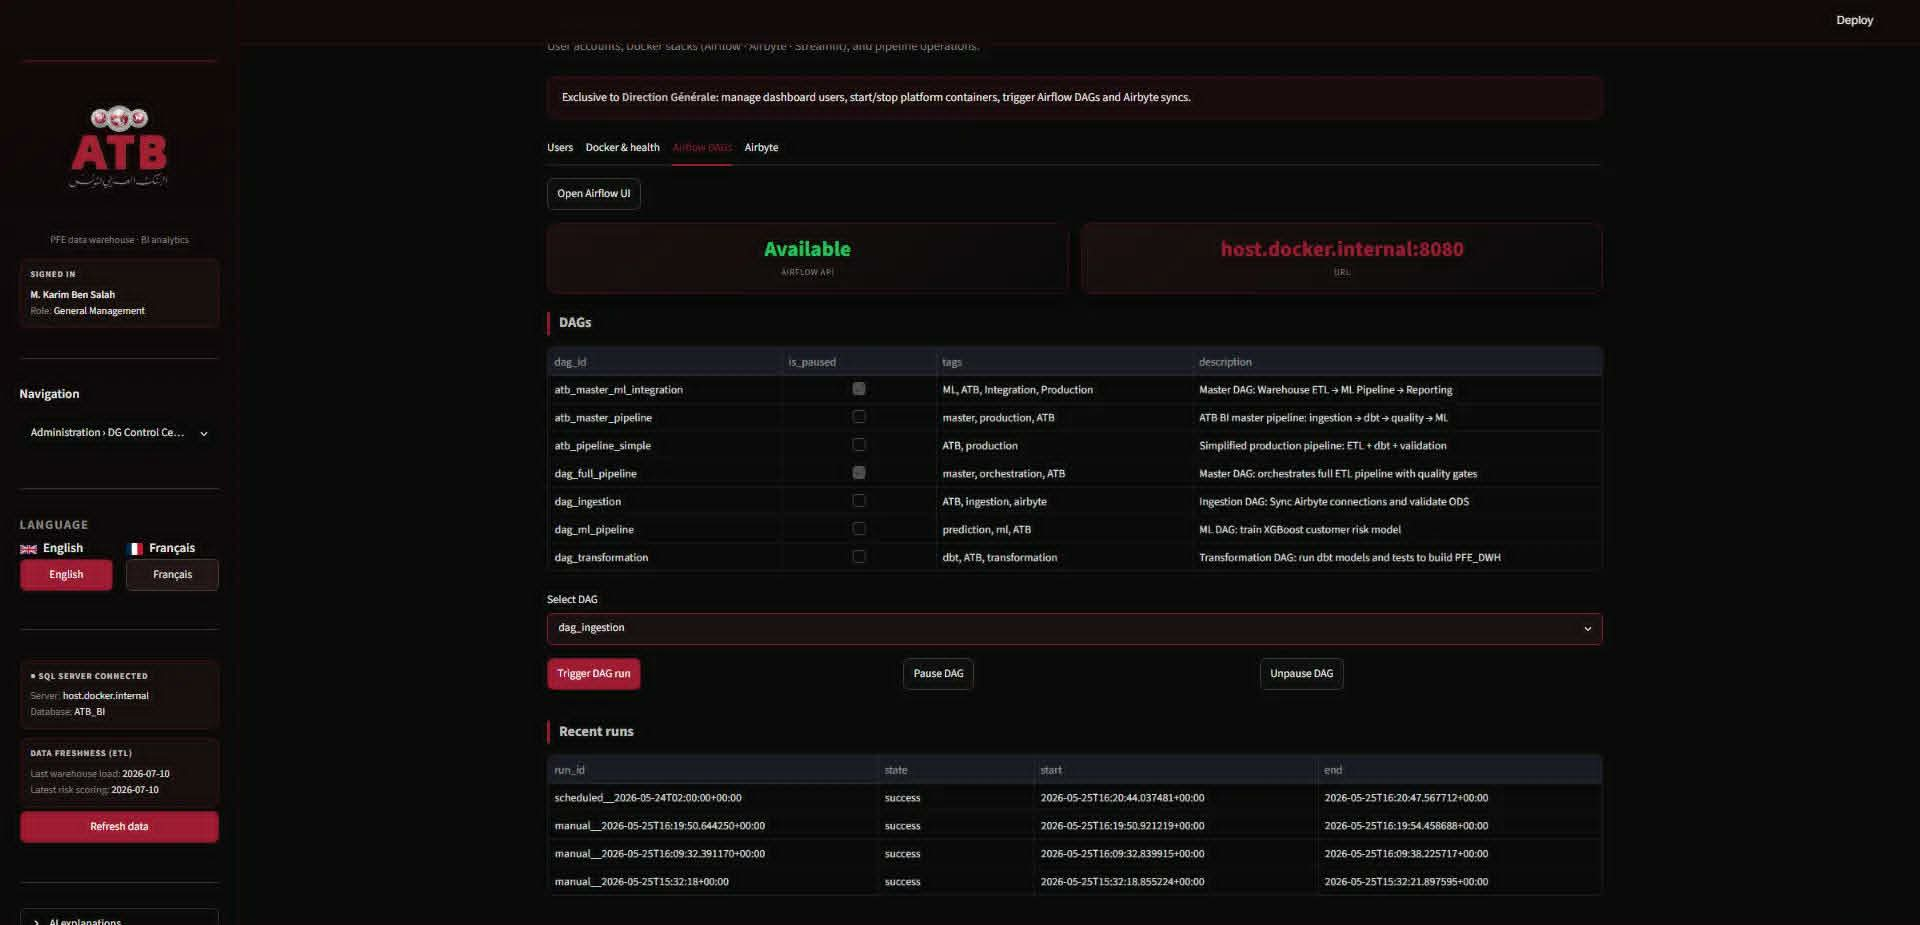
\includegraphics[width=0.9\textwidth]{figures/Streamlit Airflow Panel.png}
\caption{The Airflow monitoring panel embedded in the Streamlit}
\label{fig:streamlit_airflow}
\end{figure}

When a privileged user opens the Airflow tab within the console, the panel
automatically reaches out to the Airflow REST API and retrieves live information
about the current state of the orchestration engine. A set of status indicators at
the top of the panel immediately shows whether Airflow is reachable and healthy
a green signal means the pipeline engine is operational; a red signal triggers an
explanatory warning with guidance on how to restart the stack. Below this, the panel
displays a live table of all DAGs registered in the system, including their
current pause state, their tags, and a short description of their purpose.

\begin{figure}[H]
\centering
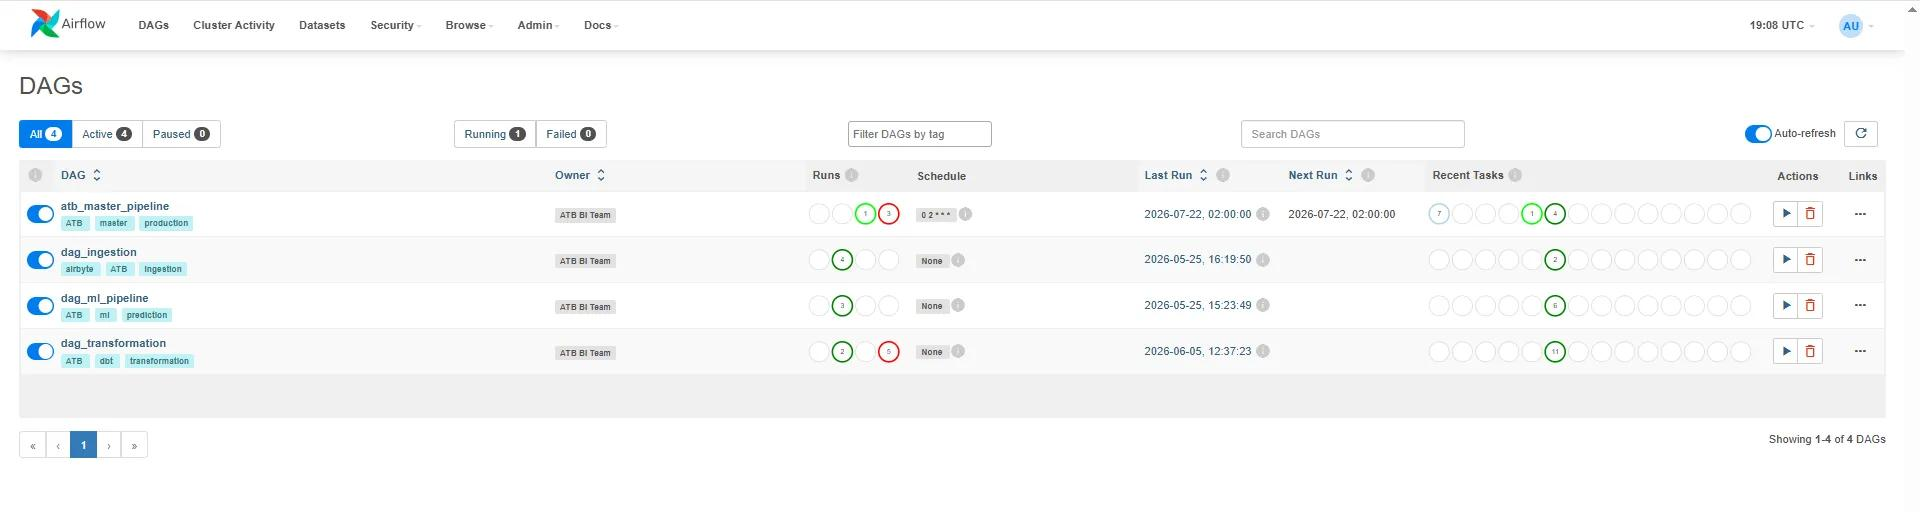
\includegraphics[width=0.9\textwidth]{figures/Airflow Dags List.png}
\caption{Live DAG registry displayed in the AirFlow}
\label{fig:airflow_dags_list}
\end{figure}

The user can select any DAG from the list and see the history of its last ten runs,
including the start and end time of each execution and its final status whether it
completed successfully, failed, or is currently running.

\begin{figure}[H]
\centering
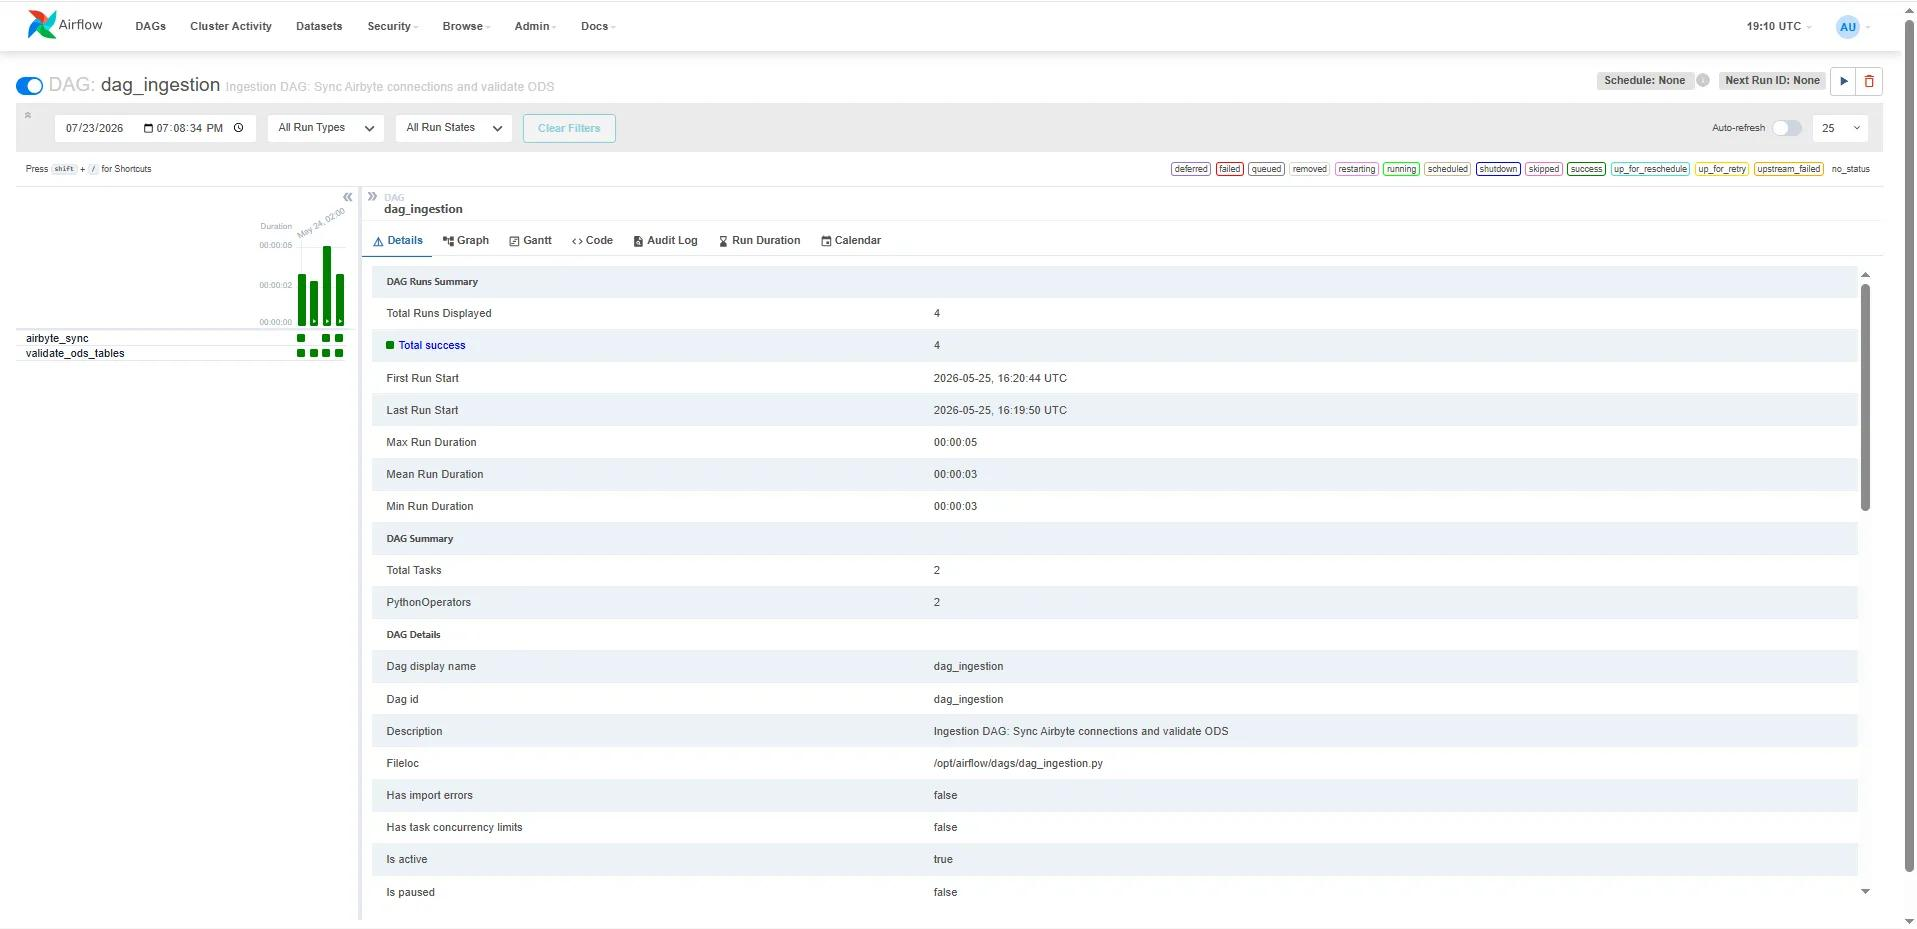
\includegraphics[width=0.9\textwidth]{figures/Dag run satus example.png}
\caption{DAG run history retrieved in real time through the Airflow API}
\label{fig:dag_run_status}
\end{figure}

\begin{figure}[H]
\centering
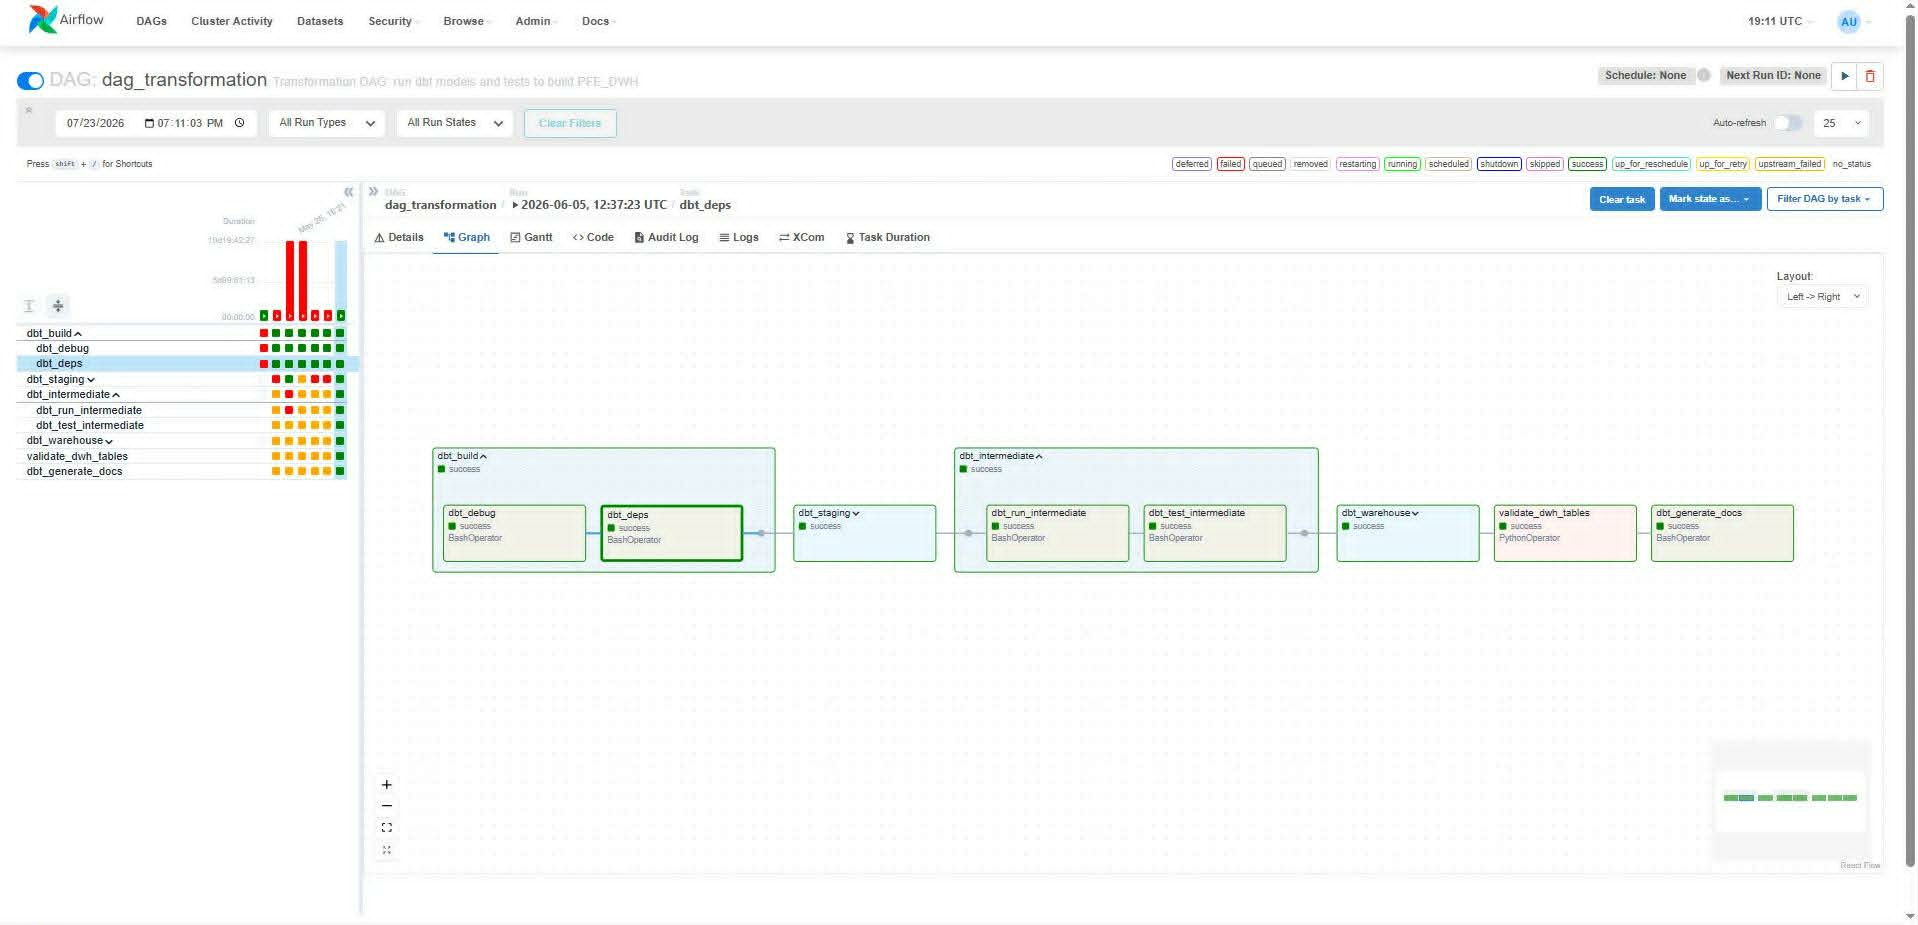
\includegraphics[width=0.9\textwidth]{figures/Full dag satus.png}
\caption{Full DAG status overview showing pipeline health across all runs}
\label{fig:full_dag_status}
\end{figure}

Beyond simple observation, the console also provides \textbf{direct control}. Three
action buttons allow authorised users to trigger a DAG manually for example, to force
a data refresh ahead of an important meeting as well as to pause or resume any
pipeline without ever leaving the Streamlit interface.

\begin{figure}[H]
\centering
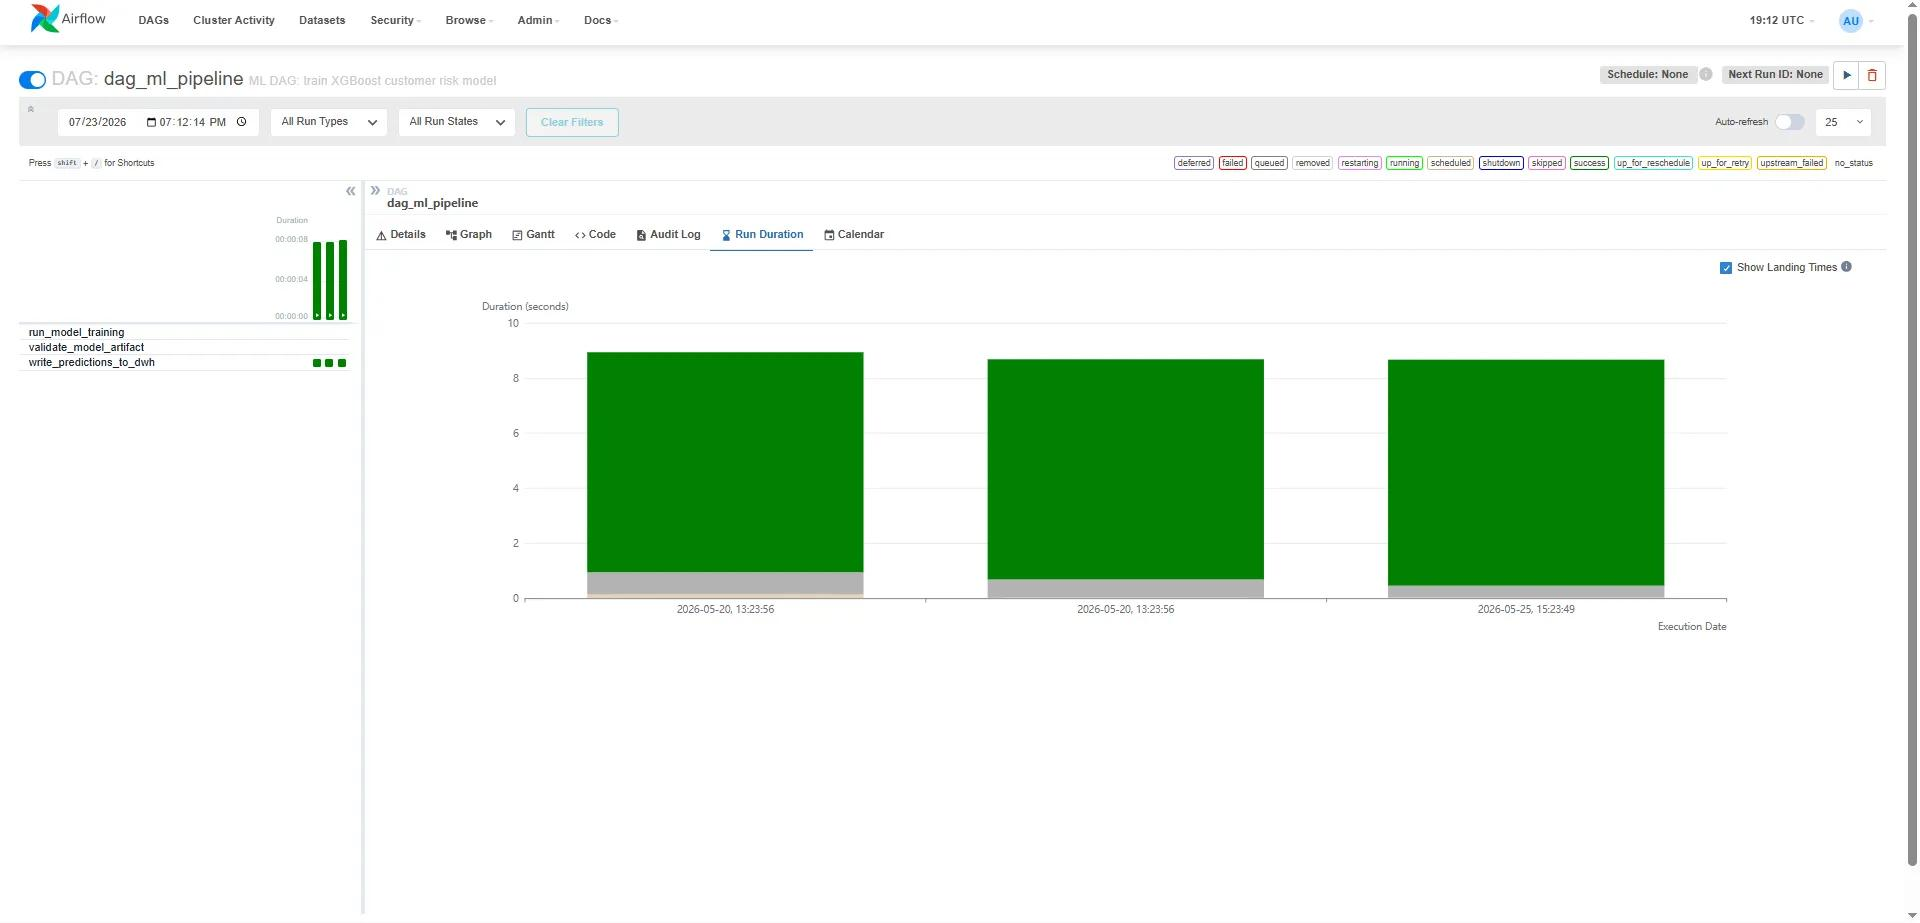
\includegraphics[width=0.9\textwidth]{figures/detailed dag action status.png}
\caption{Task-level detail view showing the outcome of each step within a DAG run}
\label{fig:detailed_dag_status}
\end{figure}

\begin{figure}[H]
\centering
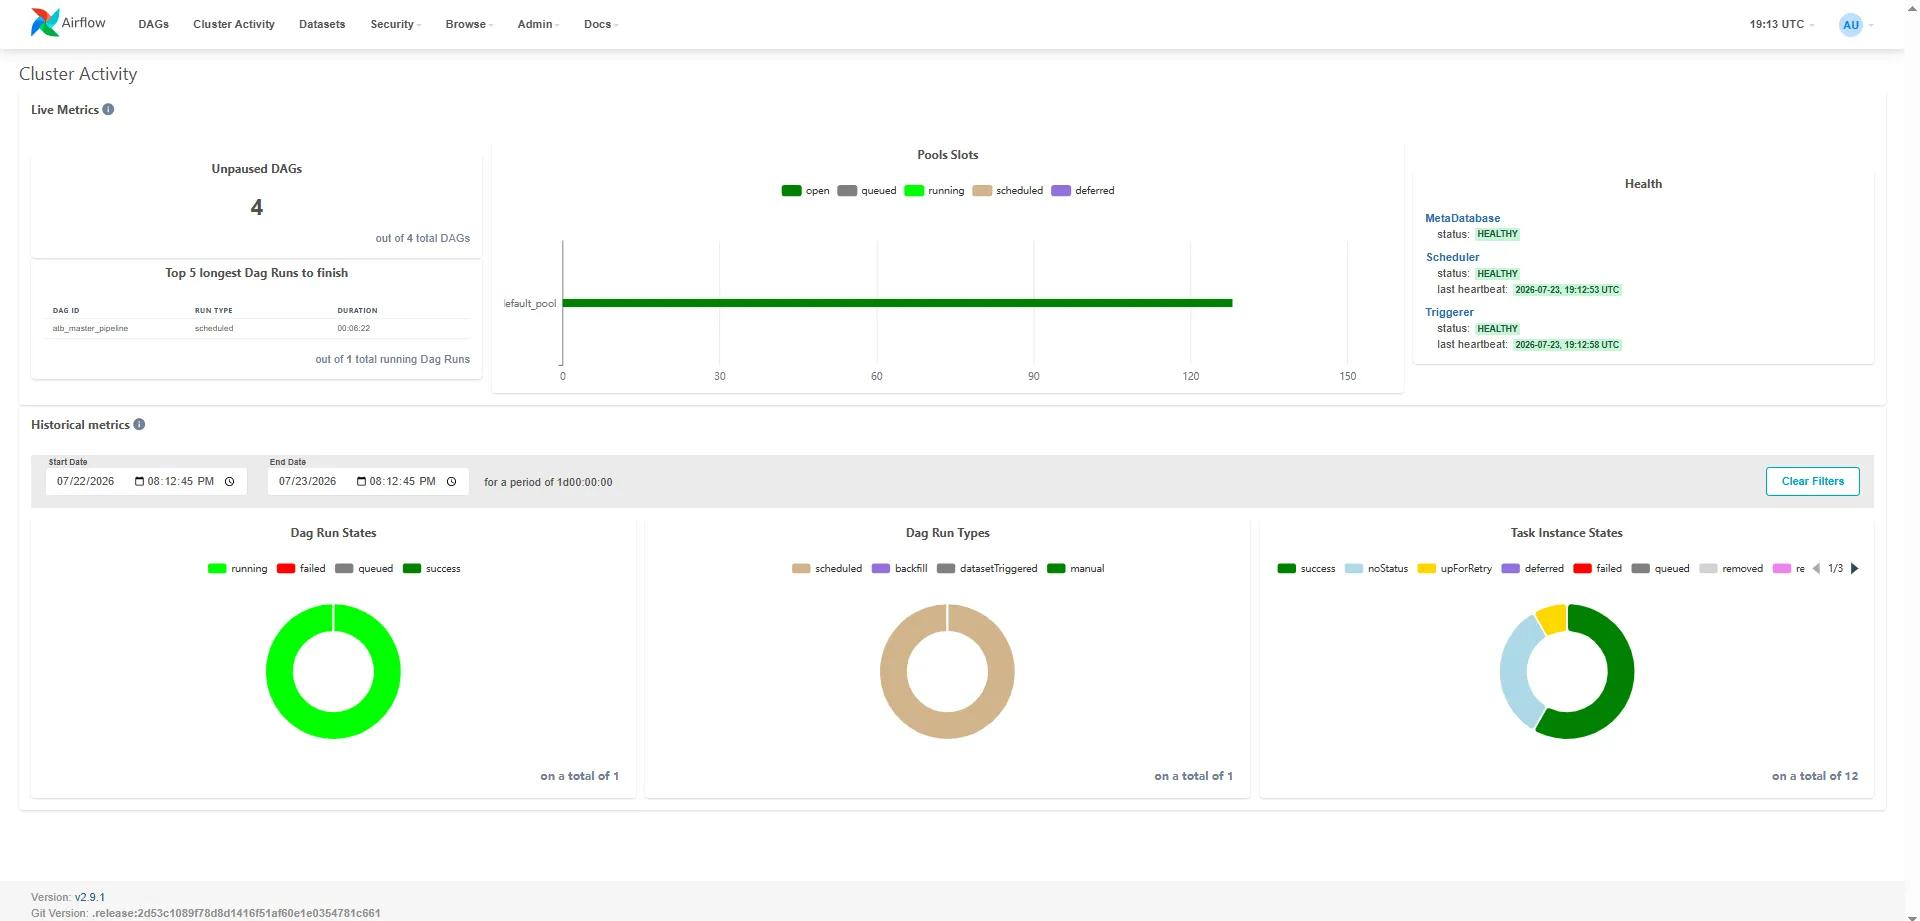
\includegraphics[width=0.9\textwidth]{figures/Airflow dashboard .png}
\caption{The Airflow web interface showing the graph view of the main pipeline}
\label{fig:airflow_webui}
\end{figure}

The same Operations Console also surfaces the status of the \textbf{underlying Docker
infrastructure}. A platform health card shows whether the Docker engine is accessible
and lists all running containers — the Airflow webserver, scheduler, triggerer, and
PostgreSQL database with their current state. Stack-level controls allow the
administrator to bring the entire Airflow stack up, down, or restart it, all through
the same unified interface. This means that the Streamlit dashboard is not merely a
reporting tool it is the central operational nerve centre of the entire data platform.

\subsubsection{Downstream Integration: From Data to Intelligence}

The pipeline does not end with data loading. Upon successful completion, it is
configured to automatically trigger the downstream machine learning pipeline, passing
control forward without any manual coordination. This creates a fully continuous,
end-to-end processing chain: raw source data enters on one side, and enriched,
ML-scored outputs emerge on the other all within a single nightly execution window,
while the organisation sleeps.

%------------------------------------------------
\section{Conclusion}

This first release established the engineering bedrock on which the entire ATB BI
platform rests. Rather than rushing toward dashboards and reports, the team invested
these two sprints in building something more fundamental: a platform that is secure
by design, autonomous by architecture, and reliable by construction.

Sprint 1 addressed the question of \textit{access}. By building a Streamlit interface
protected by role-based access control with passwords stored using salted SHA-256
hashing and user sessions scoped strictly to their organisational perimeter the
platform ensures that every interaction with banking data is authenticated,
authorised, and auditable.

Sprint 2 addressed the question of \textit{continuity}. The entire orchestration
infrastructure runs inside Docker containers, making the platform fully portable and
reproducible. Four complementary DAGs cover every aspect of the data lifecycle:
an end-to-end master pipeline that handles nightly warehouse loading and weekly
machine learning retraining, an on-demand ingestion DAG, an independent transformation
DAG, and a dedicated machine learning pipeline. The master pipeline coordinates nine
tasks across three task groups, executing every night at 02:00 UTC with a two-retry
fault-tolerance policy and integrated data quality checks that validate every foreign
key relationship before the data is made available to the business. A dedicated
monitoring panel embedded directly into the Streamlit dashboard gives authorised
administrators full real-time visibility and control over the entire platform without
ever leaving the application.
 
\textbf{Looking ahead to Release 2:} Building on this continuously operating,
autonomous foundation, the next release marks the moment where the platform
transitions from \textit{infrastructure} to \textit{intelligence}. Release 2 will
apply the GIMSI methodology to trace the complete business intelligence lifecycle:
how raw banking data extracted from seven source files travels through a rigorous
three-layer transformation process, is shaped into a governed analytical data warehouse,
and is finally brought to life on interactive Streamlit dashboards placing the right
indicators in front of the right decision-makers, at exactly the right moment.